\chapter{Formulazioni}\label{formulazioni}

In questa sezione, presenteremo due formulazioni del problema del TSP con un numero esponenziale di vincoli: la formulazione di Cut Set e Subtour Elimination. Esamineremo quali problemi portano tali formulazioni, mentre nel capitolo successivo si esaminerà un metodo e una sua variazione per gestire queste problematiche. 

\begin{figure}[ht]
	\centering
	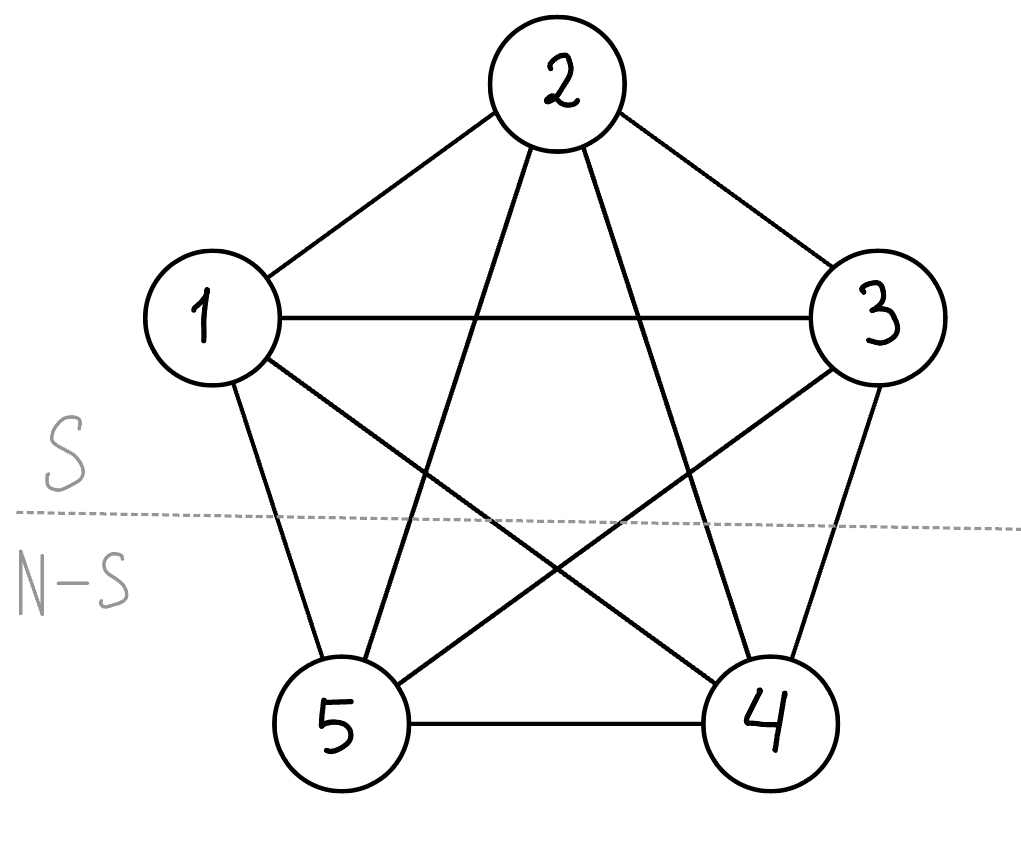
\includegraphics[width=.35\columnwidth]{images/es_taglio}
	\caption{\textit{Esempio di taglio}}
	\label{img:es_taglio}
\end{figure}

Le successive due formulazioni si basano sull'idea di utilizzare un insieme di taglio per rappresentare alcuni vincoli del TSP. Un taglio è un insieme di archi che separa il grafo \textit{G = (N, E)} in due parti disgiunte \begin{math}S \subset N\end{math} ed \textit{N - S}. 

Nelle formulazioni successive useremmo \begin{math}\delta(S)\end{math} per indicare un insieme di archi che hanno un nodo \begin{math}i \in S\end{math} e un nodo \begin{math}j \in N - S\end{math}

\[
\delta(S) = \{ (i,j) \in E: i \in S, j \notin S \}
\]

ed \begin{math}E(S)\end{math} per indicare un insieme di archi che hanno entrambi i nodi \begin{math}i, j \in S\end{math}

\[
E(S) = \{ (i,j) \in E: i \in S, j \in S\}
\]

In figura \ref{img:es_taglio} \begin{math}\delta(S) = \{ (1, 4), (1, 5), (2, 4), (2, 5), (3, 4), (3, 5)\}\end{math} ed \begin{math}E(S) = \{ (1, 2), (1, 3), (2, 3)\}\end{math}.

\section{Cut Set}
Consideriamo un grafo completo non orientato in cui i nodi rappresentano le città e gli archi rappresentano i percorsi tra le città. Definiamo le variabili decisionali binarie \begin{math}x_{i_j}\end{math} per ogni arco \textit{(i, j)}, dove \begin{math}x_{i_j} = 1\end{math} se l'arco fa parte del percorso e \begin{math}x_{i_j} = 0\end{math} altrimenti. 

\[ x_{i_j} =
  \begin{cases}
    1       & \quad \text{se} \text{l'arco \begin{math}(i, j) \in E\end{math} fa parte del percorso ottimo}\\
    0  & \quad \text{altrimenti}
  \end{cases}
\]

Inizialmente, visto che vogliamo visitare ogni nodo una volta sola, imponiamo che ognuno di questi venga "toccato" esattamente da due archi del percorso ottimo.

\[
\sum_{a \in \delta(i)} x_a = 2, \quad \forall i \in N
\]

La corrente formulazione però può portare alla individuazione di un percorso ottimo con più di un ciclo (Figura \ref{img:es_sol_disconnessa}).

La formulazione di Cut Set impone un vincolo per ogni possibile insieme di taglio che impedisce la formazione di cicli subtour. La formulazione completa del problema diventa quindi la seguente.


\[
\text{minimize} \quad \sum_{a \in E} c_a x_a
\]

\[
\sum_{a \in \delta(i)} x_a = 2, \quad \forall i \in N
\]

\[
\sum_{a \in \delta(S)} x_a \geq 2, \quad \forall S \subset N, S \ne \varnothing, S \ne N
\]

\[
x_a \in \{0, 1\}, \quad \forall a \in E
\]

Con i nuovi vincoli imponiamo che per qualunque partizione di \textit{N} in \textit{S} ed \\ \textit{N - S}, il ciclo deve 
avere almeno 2 archi tra i nodi di \textit{S} e nodi di \textit{N - S}.

\section{Subtour Elimination}
Partendo dalle stesse idee della formulazione Cut Set possiamo formulare il problema del TSP anche nel seguente modo.

Si hanno gli stessi vincoli per imporre che un nodo venga visitato solo una volta, mentre cambiano i vincoli per l'eliminazione dei cicli multipli. Riportiamo quindi solo questi vincoli in quanto la restante parte della formulazione è identica a quella di Cut Set.

\[
\sum_{a \in E(S)} x_a \leq |S| - 1, \quad \forall S \subset N, S \ne \varnothing, S \ne N
\]

Imponiamo quindi che per ogni sottoinsieme di nodi \textit{S} diverso dall'insieme \textit{N} e dall'insieme vuoto, si selezionino al più \textit{|S|-1} archi di \textit{E(S)}.


Modificando gli ultimi vincoli delle due formulazioni in \begin{math}0 \leq x_{a} \leq 1\end{math} possiamo definire il rilassamento continuo delle due formulazini con gli spazi ammissibili \begin{math}P_{cutset}\end{math} e \begin{math}P_{sub}\end{math}.
Si può dimostrare che \begin{math}P_{cutset}=P_{sub}\end{math}, cioè che le due formulazioni siano ugualmente forti.

\section{Elon Musk dimentica il teletrasporto}\label{elon_teletrasporto}

Risolvendo il TSP con le due formulazioni descritte nelle precedenti, si individua un ciclo hamiltoniano di costo minimo. La cattiva notizia sta nel numero di vincoli aggiunti per arrivare ad una soluzione connessa (quindi con un solo ciclo). 

In particolare, mentre abbiamo un numero polinomiale di  vincoli che impongono che un nodo venga visitato solo una volta, i vincoli per ottenere una soluzione connessa sono \begin{math}O(2^{|N|})\end{math}.

Elon quindi si imbatte in un problema, le due formulazioni non gli permettono di ottenere la soluzione in modo efficiente. Vorrebbe rimuovere i vincoli di connessione, ma avendo dimenticato in laboratorio il teletrasporto deve cercare una soluzione alternativa.

Nel capitolo successivo spieghiamo l'algoritmo che permette di gestire questo problema riducendolo al Problema di Assegnamento ed aggiungendo i vincoli man mano.

\newpage

\begin{figure}[ht]
	\centering
	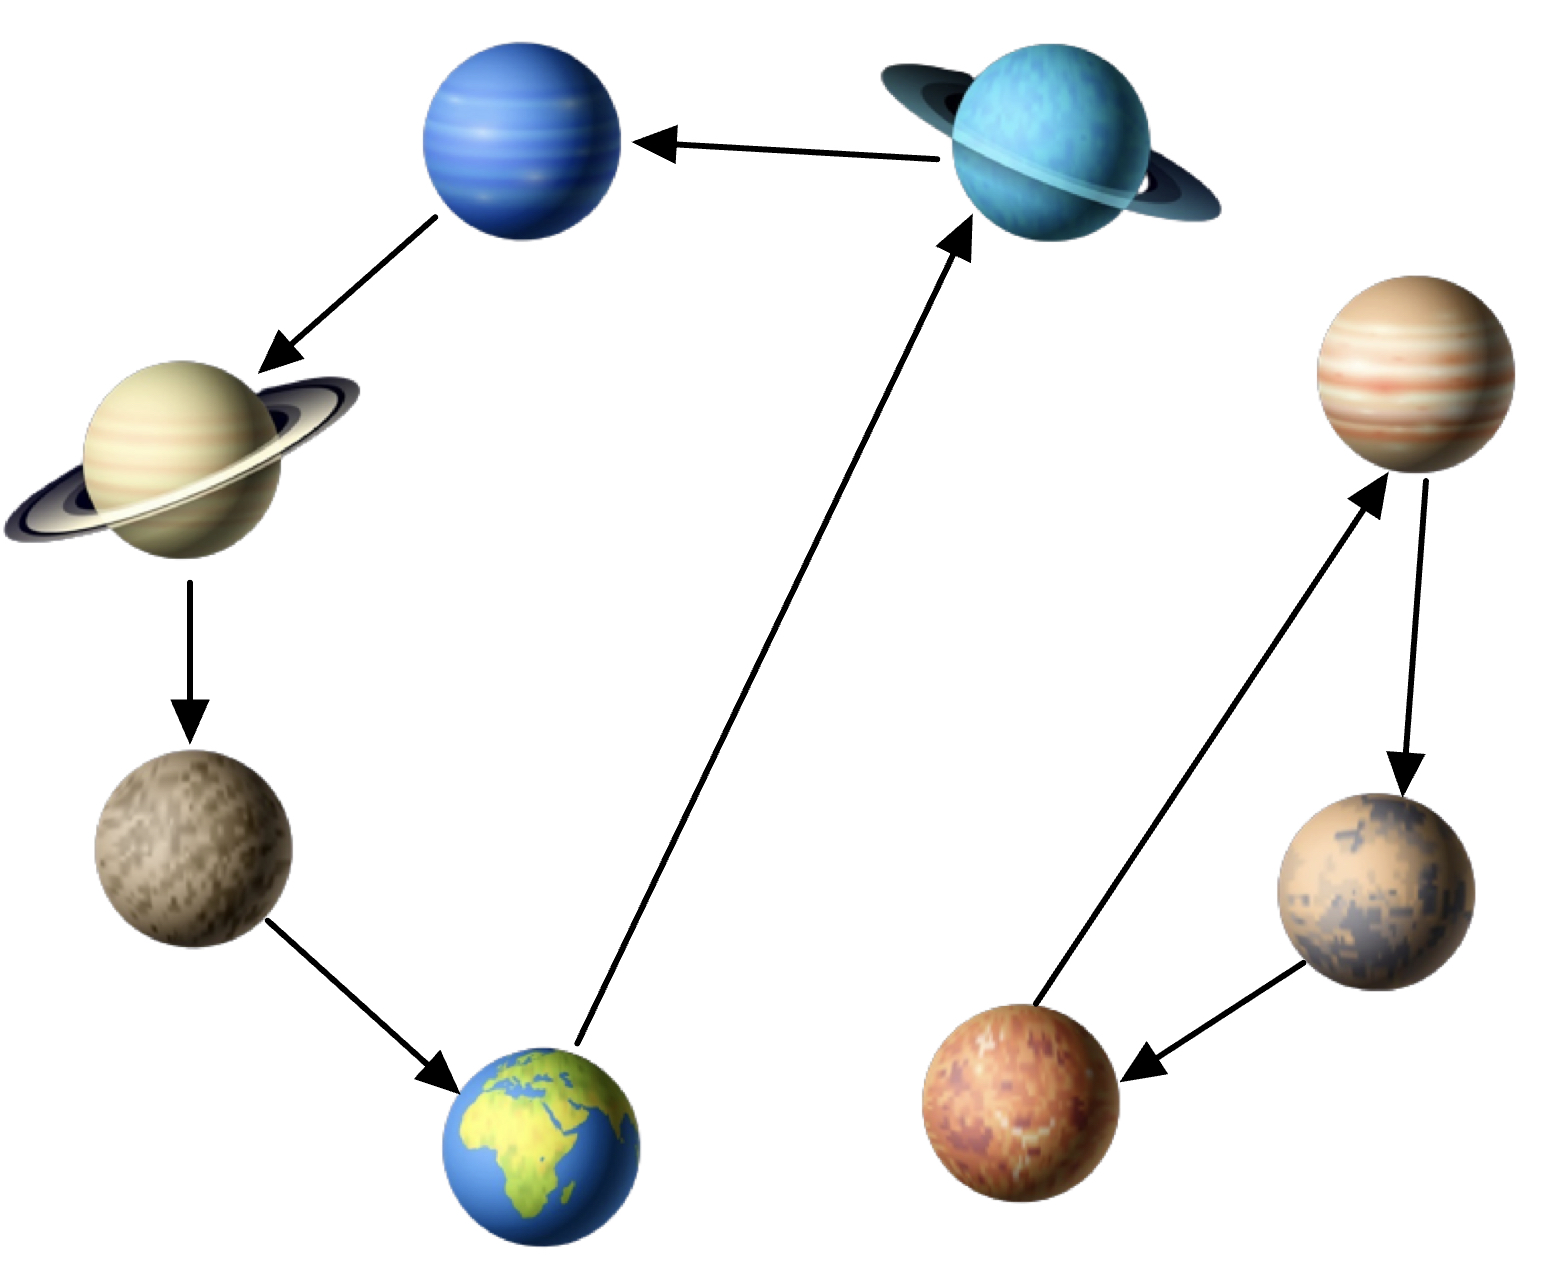
\includegraphics[width=1\columnwidth]{images/es_sol_disconnessa}
	\caption{\textit{Esempio soluzione disconnessa}}
	\label{img:es_sol_disconnessa}
\end{figure}

\begin{tikzpicture}[remember picture,overlay]
   \node[anchor=south east,inner sep=-1pt] at (current page.south east)
              {
\includegraphics[scale=0.4]{elon_thinking}};
\end{tikzpicture}

\newpage
\section{Miller–Tucker–Zemlin}\label{mtz}
Nel capitolo successivo presenteremo come possiamo affrontare il problema del TSP usando le formulazioni precedenti, cercando di aggiungere meno vincoli possibile, in quanto ci portano al problema di un numero esponenziale di vincoli per garantire la connettività della soluzione. 

In questa sezione descriviamo invece una formulazione simile, avente però un numero di vincoli polinomiale nota come la formulazione di \textit{Miller–Tucker–Zemlin} descritta in \cite{mtz}. Questa formulazione ha in comune con quella di \textit{Cut Set} e quella di \textit{Subtour Elimination} i vincoli per imporre che tutti i nodi vengano visitati e vengano visitati una volta sola.

\[
\sum_{i = 1}^{|N|} x_{i_j} = 1, \quad  i = 1, \dots, |N| 
\]

\[
\sum_{j = 1}^{|N|} x_{i_j} = 1, \quad  j = 1, \dots, |N|
\]

Abbiamo però delle variabili decisionali nuove \begin{math}u_i \in \mathbb{R}\end{math} per \begin{math}i = 1, \dots, n\end{math}. Le variabili aggiuntive vengono utilizzate per dare un ordine a tutti i nodi (\begin{math}u_i\end{math} rappresenta la posizione del \textit{i-iesimo} nodo nel percorso). Con i seguenti vincoli, queste variabili vengono utilizzate per assicurare un ciclo hamiltoniano valido. 
Otteniamo questo risultato assicurandoci che \begin{math}u_j \ge u_i + 1\end{math} quando l'arco associato a \begin{math}x_{i_j}\end{math} viene selezionato. 
Il problema di questa formulazione è quella di avere un rilassamento molto forte della soluzione.

\[
u_i - u_j + (n-1)x_{i_j} \leq n - 2, \quad \forall i \ne j = 2, \dots, n
\]

\[
u_i \in \mathbb{R}, \quad \forall i = 2, \dots, n
\]
